% Orthogonal projection of x onto a plane W: x = Px + (x - Px), with x - Px perpendicular to W.
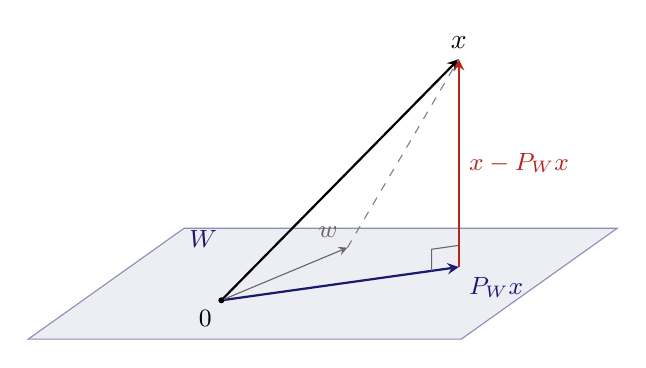
\begin{tikzpicture}[scale=1.1,>=stealth,x={(1cm,0cm)},y={(0.45cm,0.32cm)},z={(0cm,1cm)}]
\filldraw[fill=MidnightBlue!8,draw=MidnightBlue!50] (-1.6,-1.4,0) -- (3.4,-1.4,0) -- (3.4,2.6,0) -- (-1.6,2.6,0) -- cycle;
\node[MidnightBlue,font=\small] at (-1.2,2.2,0) {$W$};
\coordinate (O) at (0,0,0); \coordinate (P) at (2.2,1.2,0); \coordinate (X) at (2.2,1.2,2.4);
\coordinate (W1) at (0.6,1.9,0);
\draw[->,thick] (O) -- (X) node[above] {$x$};
\draw[->,thick,MidnightBlue] (O) -- (P) node[below right,font=\small] {$P_Wx$};
\draw[->,thick,BrickRed] (P) -- (X) node[midway,right,font=\small] {$x-P_Wx$};
\draw[black!60] (2.2,1.2,0.25) -- (1.95,1.06,0.25) -- (1.95,1.06,0);
\draw[->,black!60] (O) -- (W1) node[above left,font=\small] {$w$};
\draw[dashed,black!50] (W1) -- (X);
\fill (O) circle (1pt) node[below left,font=\small] {$0$};
\end{tikzpicture}
